\chapter{Fast Radio Bursts}\label{ch:frb}

\par The domain of Radio Astronomy is full of surprises. 
It all started with the serendiptious detection of \emph{a bright millisecond radio burst}~\cite{first_frb} in the archieval data which brought into light, the existence of short time-scale, extremely energetic radio signals, possibly originating from beyond the galaxy. 
These signals are called \emph{Fast Radio Bursts (\frb{})} and the search for these signals forms the crux of this thesis.

\par The first discovered \frb is the~\cite{lorimerburst} in $2001$, colloquially known as the \emph{Lorimer Burst}. 
Many theory papers followed but there was no corroborative detection. In the lack of which, skeptisim arose~\cite{burke_doubt}. 
Prior to that~\cite{old_m87_bursts} detected \frb-like pulses with \dm as high as $5\times 10^3$ \pc originating from \textt{M87}. So, these may very well have been the first detection of \frb~s but due to the limited time/frequency resolution, no substantiative evidence could be established. 

\par Astronomers were not wrong in their dubious nature. Their experience with another specie of signals called Perytons~\cite{perytons} justifies it. Named after the mystical hybrid bird, these signals were actually caused by the microwave on the observatory site. The premature opening of the microwave door shuts off the magnetron abruptly, which produces a dispersed-like signal which was then picked up by the radio telescope.
This put more shade on the celestial nature of the \emph{Lorimer Burst}.

\par But then came as a surprise, ~\cite{danburst4} in $2016$ which reported $4$ such bursts and thus set in stone the existence of such species. 
Now, four years and sophisticated advancements in observatory technologies later, the number of \frb{}s detected is in thousands. The details of this story will be discussed in \autoref{sec:detect_so_far}.

\par Given the amount of shear energy emitted in these bursts, astronomers were not wrong in maintaining an innate assumption that these events were result of a cataclysmic event. And by the very nature of such events, \frb{}s were not expected to repeat. And then came as a surprise, \frb{121102} in $2012$, which repeated in time.
Over the years since its discovery, \frb{121102} is perhaps the most studied \frb{} with observations done from meter wavelength to milli-meter wavelength. See~\cite{sptlier}.

\par Astronomy wouldn't be full of surprises, if \frb{121102}~ was the only repeating \frb{}~ found. In $2019$,~\cite{chime_repeaters} found $4$ repeating \frb{}s (henceforth called repeaters) using the Canadian Hydrogen Intensity Mapping Experiment (CHIME) telescope which prompted a fresh set of theories to emerge to explain the same.

\par All the discovered \frb{}s are catalogued in \textt{FRBCAT}~\cite{frbcat}. All the theories of \frb{}s are also catalogued in \textt{FRB-theorycat}~\cite{frbtheorycat}.


\section{What are FRBs?}

\par Before we go into \frb{}s. It is crucial to establish certain groundwork known in a radio astronomy setting. 
First being the data representation format widely used: filterbank in~\autoref{ssub:fb}. 
Second being the phenomenon of dispersion which affects all the radio signals propagating through the space and reaching the radio telescope. 
This will be covered in detail in~\autoref{ssec:dis}.

\par Then, in~\autoref{ssub:dis}, \frb{}s are characterized.

\subsection{Filterbank}
\label{ssub:fb}

\par A popular data representation format for radio astronomers is the time frequency bins, known as filterbank, where every bin has one or more of the four Stokes parameter. In a typical setting, of the four, only the Stokes I is recorded.
Any radio astronomy setup involves a frequency band $[\nu_{\rm LOW}, \nu_{\rm HIGH}]$ of interest discretized into \texttt{NCHAN} frequency channels, yielding frequency channel width, denoted by \texttt{FOFF}, as bandwidth divided by the number of channels.
Time samples are sampled at a suitable Nyquist Sampling rate commensurate with the bandwidth $\nu_{\rm HIGH} - \nu_{\rm LOW}$. Let the sampling rate be \texttt{TSAMP}.

\par With the above definitions in place, starting off with voltage samples, by applying Short Time Fourier Transform and consequently taking magnitude (essentially Stokes I), filterbank is produced. In practise, a suitable digitization scheme is employed and data is digitized to \textt{NBIT} bits per sample.
Every consecutive time sample is separated by \texttt{TSAMP} in time and every consecutive frequency sample is separated by \texttt{FOFF}.
This representation makes it easier to look at the time frequency variations and hence is popular.

\subsection{Dispersion}
\label{ssub:dis}

\par Imagine sending sunlight through a prism. It is common knowledge to expect rainbow emanating from the prism. 
This same phenomenon is what brings a rainbow after the rain if the Sun is up. The physics behind this as follows:
White light is made up of the seven colors. And, when white light goes through the prism, distinct color components get separated,
and a rainbow is observed. 
This phenomenon is called dispersion and is not just valid for white light (or, visible band of electromagnetic spectrum). 
Of course, the properties of the prism changes when going to a different band of electromagnetic spectrum. But, any part of the electromagnetic spectrum can get dispersed and its frequency components can get separated. And since different frequencies of visible light correspond to different colors, we see colors of a rainbow.

\par Radio waves propagating in space also suffer the same fate.\emph{Prisms} here are plasma made of electrons in the space. 
This plasma exists in the line of sight between the source and the observatory. A better understanding of the dispersion can be made by using hte filterbank representation. Dispersion causes progressively lower frequencies to receive the signal latter than their higher frequency counterpart. See fig.

\par The time difference (also known as dispersion smearing) is calculated with the~\ref{eq:dispersion}. The \dm appearing in the equation is called the Dispersion Measure which is a measure of the electron number density in the column along the line of sight.
\begin{equation}
\label{eq:dispersion}
\Delta t = {\rm DM} \times 4.15 \times 10^{-3} \big[  \frac{1}{\nu^2_{\rm LOW}} - \frac{1}{\nu^2_{\rm HIGH}} \big]\ {\rm s}
\end{equation}
This effect of dispersion is to be corrected for any analysis and the process is called de-dispersion. More details about de-dispersion will be covered in~\autoref{chap:inst, }.

\par Dispersion is purely a propagation effect. Thus, amount of dispersion provides a good marker of distance. There are two models for electron distribution in the galaxy, NE2001~\cite{ne2001} and YMW~\cite{ymw16}. With the help of a model, given a pointing in Galactic coordinates ($l$, $b$), the \dm contribution by the Galaxy can be estimated. This model becomes useful later when talking about \frb{} origin in following sections. 

\subsubsection {De-dispersion}
\label{sssub:dd}

\par In order to compensate for the dispersion effect, de-dispersion is performed. The de-dispersion is a computationally intensive process.
\par With a filterbank, de-dispersion can be straightforward where frequency channels are time-shifted can do the job. 
However, this does not negate dispersion effects in the frequency channel, leading to what is called the in-channel smearing.
Mathematically, it can be derived by using small bandwidth approximation to~\autoref{eq:dispersion}. 
See~\autoref{eq:inchannel} where $\Delta \nu$ is the channel bandwidth and $\nu$ is the frequency of the top end of the channel.
\begin{equation}
\label{eq:inchannel}
\Delta \tau = {\rm DM} \times 4.15 \times 10^{-3} \big[  \frac{\Delta \nu}{\nu^3}  \big]\ {\rm s}
\end{equation}

\subsection{Characteristics}
\label{ssub:frb}

\par \frb{}~s are short time-scale ($\sim$ ms), bright ($0.001 - 100$ Jy), broadband (present in \emph{almost} all frequency channels) and extremely dispersed (very large \dm) radio signals. 
The most distinctive feature of an \frb{}~ is its \dm which is many fold more than the galaxy could contribute. The galaxy contribution to a signal detected at an observatory is calculated using the pointing information (at the time of detection) and using an eletron density model as discussed in~\autoref{ssec:dispersion}.

\par To further appreciate the high \dm of \frb{}~, the \dm and $\frac{\rm DM}{{\rm DM}_{\rm Max}}$ are plotted. DM$_{\rm Max}$ is maximum galactic contribution for the given pointing. See ~\autoref{fig:dmdmax} also~\autoref{petroff_survey, palfa_frb}. Clearly, all the \frb{}s are atleast multiple times the galactic contribution. This inference, combined with the understanding that \dm~ is a proxy for distance, provides evidence that \frb{}s origin from extra-galactic and of cosmological nature.

\begin{figure}
\label{fig:dmdmax}
	\centering
	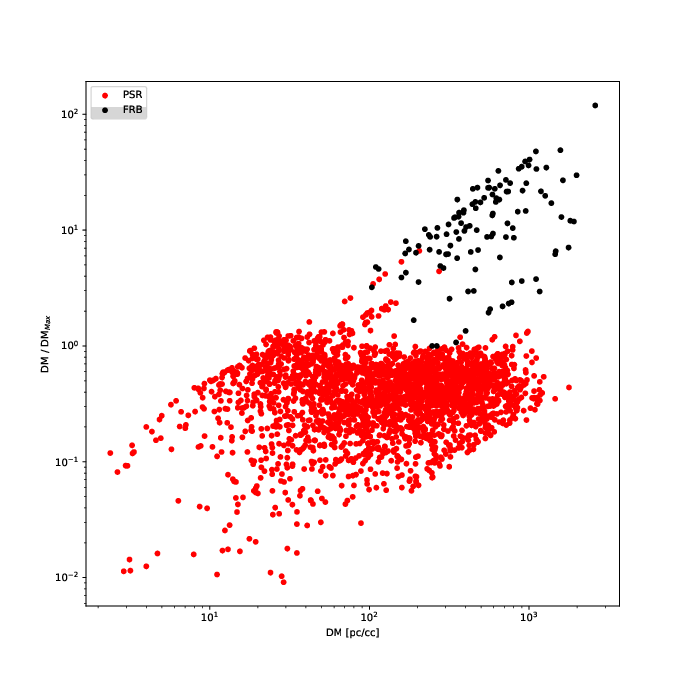
\includegraphics[width=0.8\textwidth, keepaspectratio]{dm_dmax.png}
\caption{\dm v/s $\frac{\rm DM}{{\rm DM}_{\rm Max}}$. An updated version of~\cite{petroff_survey, palfa_frb}.}
\end{figure}

\par 

\section{Detections so far}

\par Using the catalogued \frb{}s from \textt{FRBCAT} mentioned in the start of the chapter, a brief summary of the \frb{}s population is given.
Firstly, \autoref{fig:frbtime} summarizes the \frb{}s detected by various instruments over time. \autoref{fig:frbsky} shows the sky distribution of the \frb{}s. One-off events are marked by blue circles and repeaters are marked by red crosses. If \frb{}s are indeed extra-galactic, the sky distribution would be isotropic.

\begin{figure}
	\label{fig:frbtime}
	\caption{Population of \frb{}s over time. The exponential trend is what drives \vf.}
\end{figure}

\begin{figure}
	\label{fig:frbsky}
	\centering
	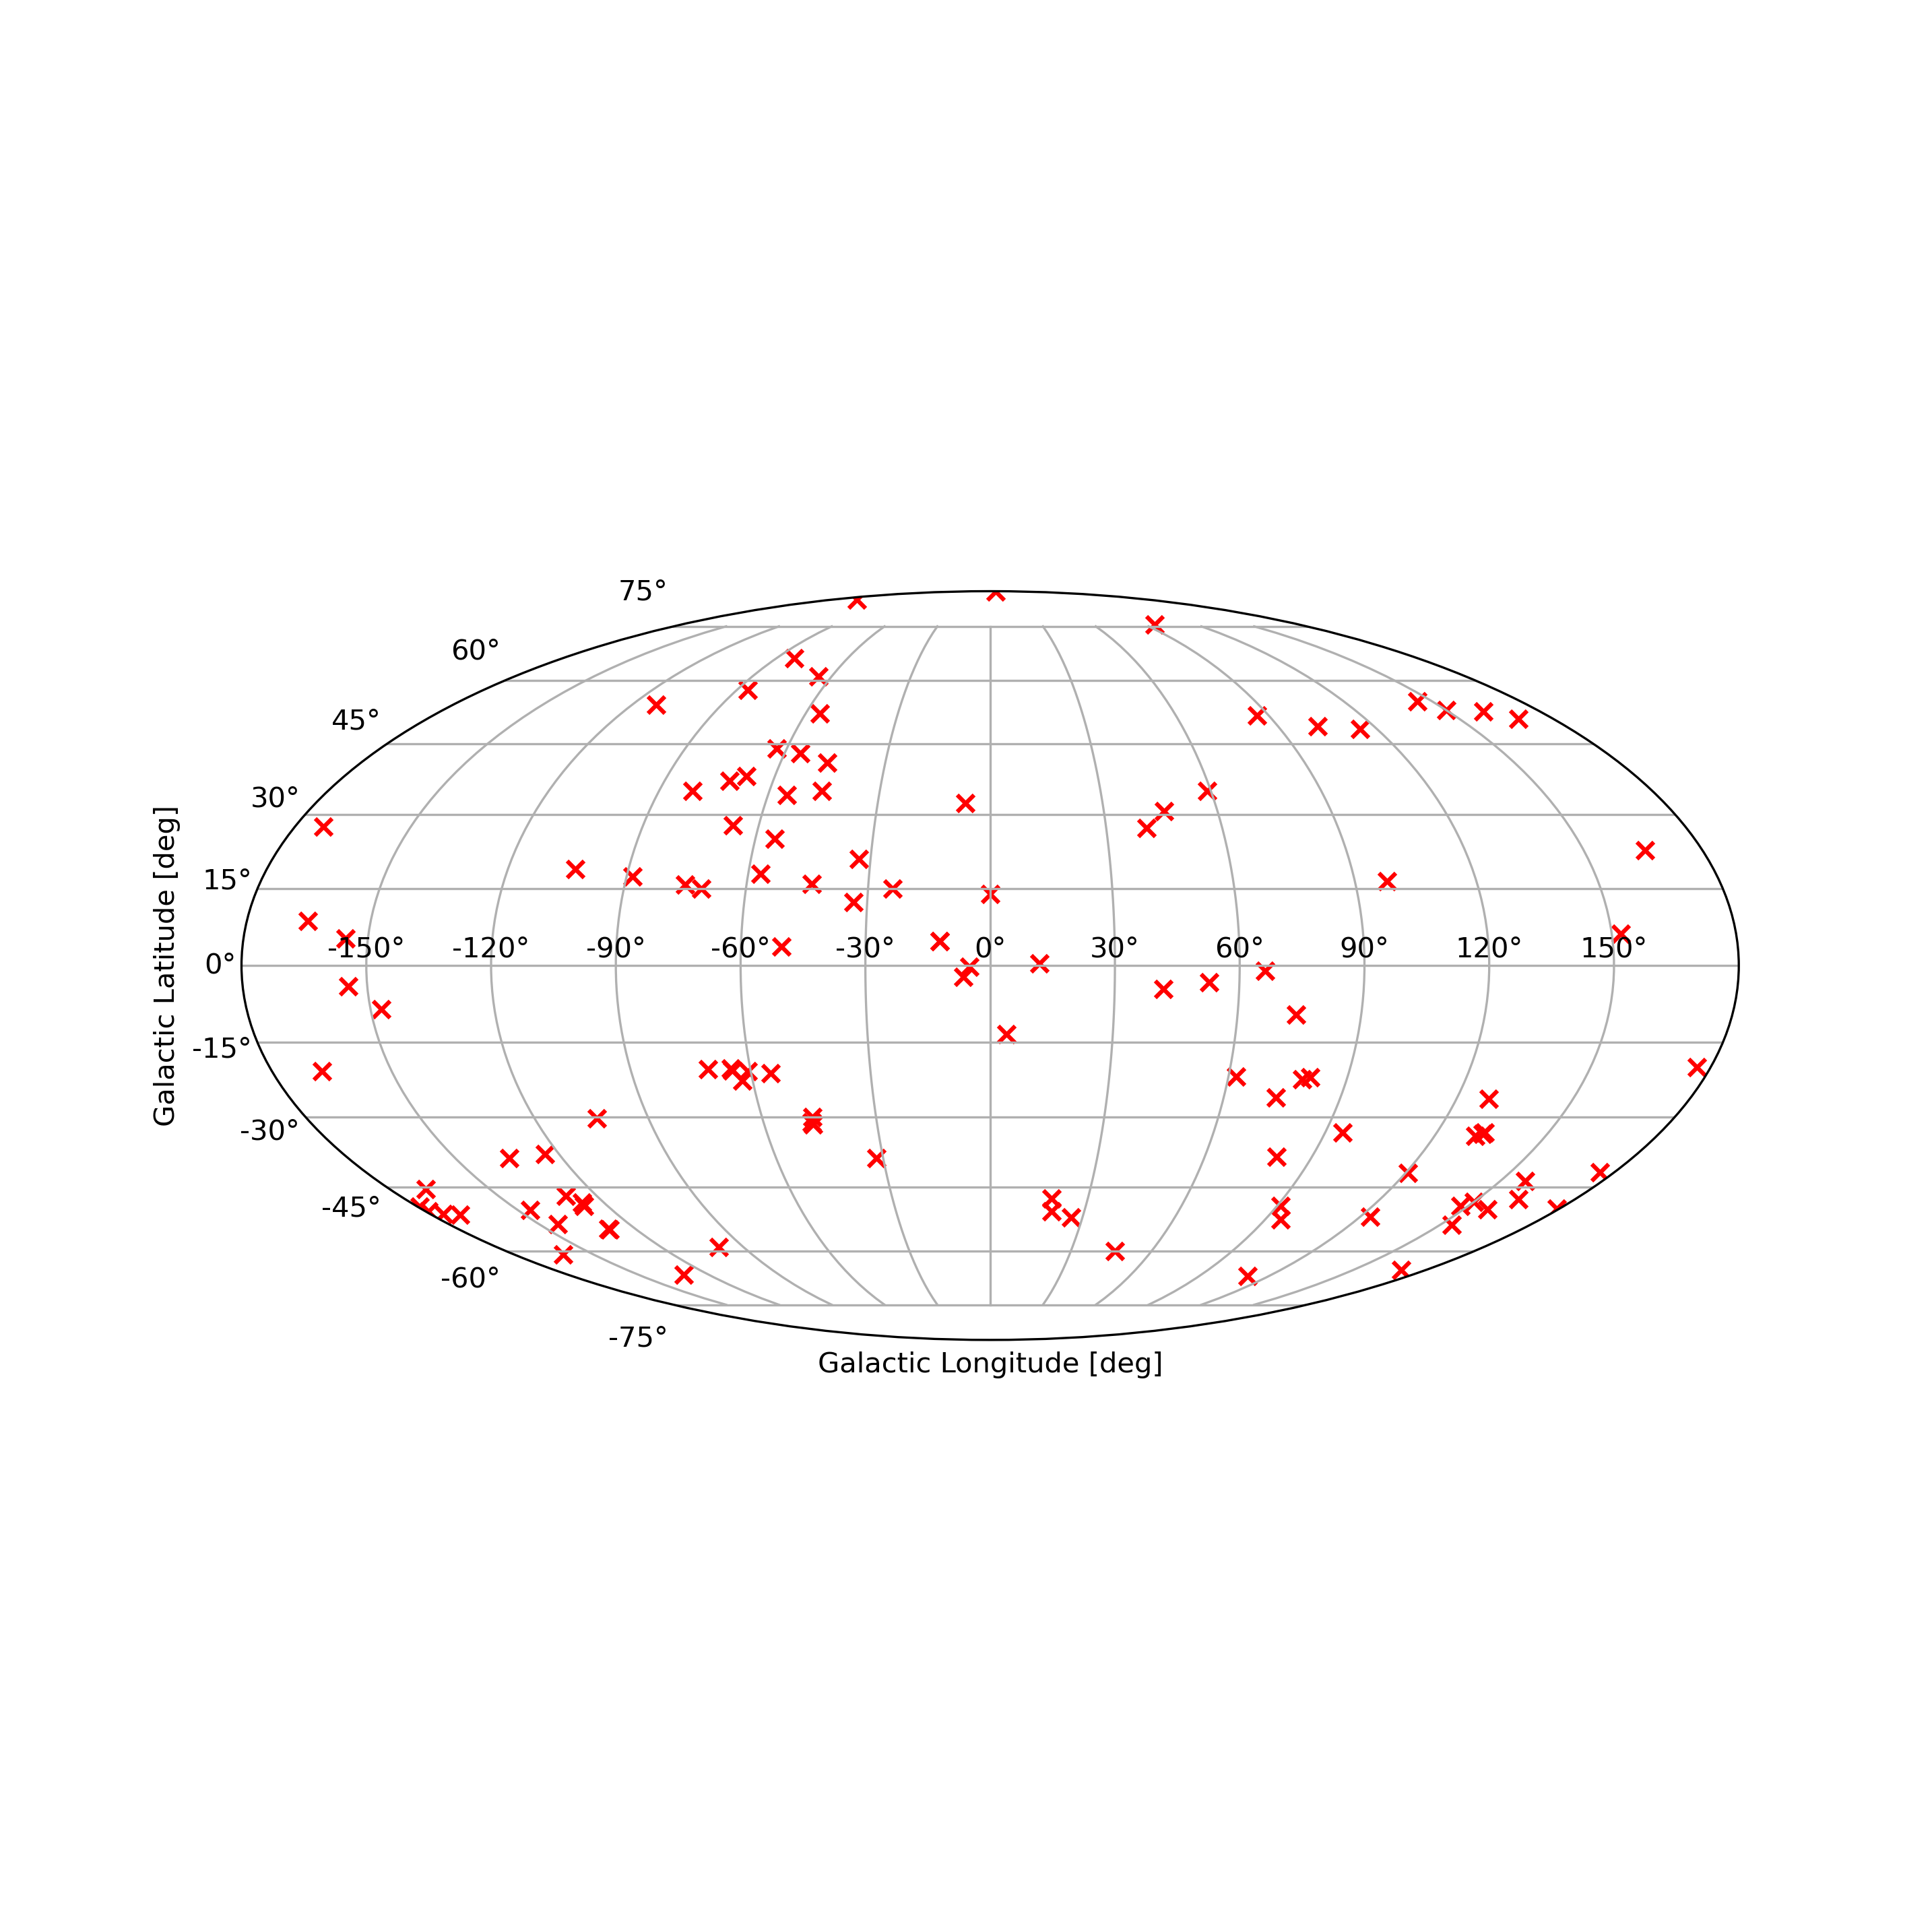
\includegraphics[width=0.8\textwidth, keepaspectratio]{frb_skymap.png}
	\caption{Population of \frb{}s over sky. }
\end{figure}

\par Lastly, no introduction of \frb{}s is complete without rate calculations. With each survey for these signals, a rate of \frb{}s is computed in the units of per-day-per-sky to quantify the yield of the survey. This metric is rudimentary and shows how much is actually known about them. ~\autoref{tab:frbrates} captures the event rates published by various surveys.

\begin{table}
	\label{tab:frbrates}
	\caption{\frb{}~ event rates with frequency band.}

\end{table}

\section{Thesis outline}


\subsection{VLITE}

\par This study is a part of the \texttt{VLA Low Frequency Ionospheric and Transient Experiment (\vlite)}. 
\vlite is a commensual observing system of the Karl Janksy Very Large Array radio telescope~\cite{vla} upon which \vf is based. 
Hence before describing the outline, the \vlite system is described here.

\par A selected subset of \vla antennas are fitted with low frequency receiver units at the casegrain feed. 
Receivers are tuned to operate in $320-384$ MHz giving a bandwidth of $64$ MHz. Due to the Mobile Users Operating System (MUOS) of the Department of Defense, the higher end of the band receives a lot of Radio Frequency Interference (RFI), as a result, the frequency band is cut off at $361$ MHz. Nevertheless, the voltage data is sampled at $128$ Mhz (the Nyquist frequency of $64$ MHz bandwidth).
\par The sampled data from each of the antenna is multicast on the observatory intranet using the User Datagram Protocol (UDP) in the form of VLBI Data Interchange Format (VDIF) packets. At the time of writing, there are $16$ \vla antennas participating in \vlite. \vlite also consists of $12$ compute nodes with one login node which are interconnected by an Infiniband network~\cite{infiniband}. 
Each compute node houses nVIDIA Graphical Processing Units (GPUs) for all the signal processing and also has a $500$ GB Solid State Disk (SSD) installed.

\par This infrastructure is shared by two different pipelines: \vlite-SLOW and \vf. \vlite-SLOW is an imaging pipeline which produces short time skymaps and is not the focus of this thesis. \vf is a search pipeline which searches for \frb{}s.

\subsection{VLITE as an FRB search engine}
\label{ssub:vfrb}
\par \vlite~is a well suited engine to detect \frb{}s. The salient features are summarized here:
\begin{description}
	\item[Commensal] 
		\vlite~ being a commensal system has uncontested access to the data from the \vla antennas.
		This leads to extremely large onsky times which are the times actively looking for signals of interest.
	\item[Large field-of-view (FOV)]
		Each \vlite~ antenna is a $25-$meter dish with center frequency of $350$ MHz ($0.85$ meters in wavelength). 
		The diffraction limit of each antenna is $\frac{\lambda}{D}$ where $D$ is the diameter of the dish and $\lambda$ is the wavelength.  
		\vlite~ achieves a diffraction limit of $0.034$ radians or $1.94^o$. 
		An $\sim 2^o$ FOV covers a large portion of the sky. 

	\item[Sensitivity]
		\vlite~ employs $16$ antennas.
		Use of a large number of antennas helps in reducing the overall background noise and thereby increases the sensitivity of the signal.
	
	\item[Inteferometer]
		An inteferometer is a type of radio telescope with spatially separated antennas. 
		The spatial separation helps produce a delay between any pair of antennas which is then used to triangulate (localize) the source of the signal. 
		\vla~ is an interferometer. And, hence, \vlite~ is too.
		Given how far the \frb{}s are originating from, any task of localizing the cause/source of the signal is hindered by the inability to precisely identify the particular pointing in sky from where the signal has originated.
		Here lies the strength of \vlite~.
\end{description}

\par With the help of these features, \vlite~endevors to be a \emph{FRB localizing search engine}. 

\subsection{Outline}

\par The goal of the study is to establish and start a search campaign making use of the commensual observation system \vlite of the \vla radio observatory.
With this in mind, a robust yet efficient realtime search pipeline was designed and coded (see~\autoref{chap:inst}).
The data taken became a part of VLITE-Fast Pathfinder Survey (\vfpfs). The data is discussed in great detail in~\autoref{chap:data}.
A completeness analysis, in which pure random noise was sent through pipeline, is performed to test the noise response of the pipeline. In addition, artificial signals of interest were inserted into the pipeline for testing the pipeline in a controlled environment. 
The data products yielded by \vfpfs and the controlled testing have been used to develop an Aritificial Intelligence (AI) which will be covered in~\autoref{chap:ml}.
The resulting AI solution is used to vet through the entire \vfpfs dataset to identify any unknown signal missed previously. Results of the AI analysis are also reported in the same chapter. 


